\myslide{Source Code - Highlighting}
{
  Freie Identier und Typ-Namen werden in den Source Code Editoren hervorgehoben.
  Dies ist nützlich, da diese meist auf eine fehlerhafte Eingabe zurückzuführen
  sind. In diesem Fall ist der Identifier \glqq add\grqq\ und der Typ-Name 
  \glqq t\grqq\ frei vorkommend.\\
  \begin{tabular}{p{12.1cm}@{}p{12.1cm}@{}}
    \begin{center}
      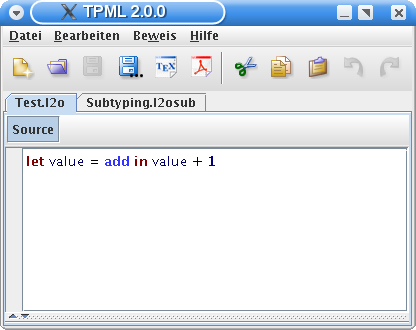
\includegraphics[width=11.6cm]{images/sourcecode_free_identifier.png} 
    \end{center}
    & 
    \begin{center}
      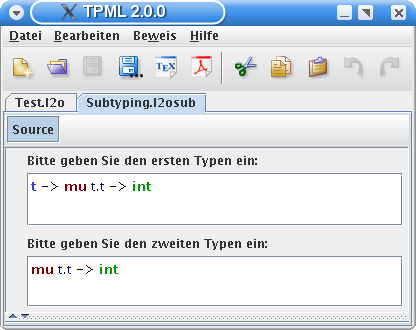
\includegraphics[width=11.6cm]{images/sourcecode_free_typename.png}
    \end{center}
  \end{tabular}
}